% A LaTeX (non-official) template for ISAE projects reports
% Copyright (C) 2014 Damien Roque
% Version: 0.2
% Author: Damien Roque <damien.roque_AT_isae.fr>

\documentclass[a4paper,12pt,openany]{report}
\usepackage[utf8]{inputenc}
\usepackage[T1]{fontenc}
\usepackage[english]{babel}
\usepackage{a4wide}
\usepackage{graphicx}
\usepackage{float}
\usepackage[sort, numbers, square, super]{natbib}
\graphicspath{{images/}}
\usepackage{ifthen}
\usepackage{ifpdf}
\ifpdf
\usepackage[pdftex]{hyperref}
\else
\usepackage{hyperref}
\fi
\usepackage{color}
\hypersetup{%
colorlinks=true,
linkcolor=black,
citecolor=black,
urlcolor=black}

\renewcommand{\baselinestretch}{1.05}
\newcommand{\code}[1]{\texttt{#1}}%code snippets
\usepackage{fancyhdr}
\pagestyle{fancy}
\fancyfoot{}
\fancyhead[R]{\bfseries\nouppercase{Progress Report I}}
\fancyhead[L]{\bfseries\nouppercase{\rightmark}}
\setlength{\headheight}{15pt}

\let\headruleORIG\headrule
\renewcommand{\headrule}{\color{black} \headruleORIG}
\renewcommand{\headrulewidth}{1.0pt}
\usepackage{colortbl}
\arrayrulecolor{black}

\fancypagestyle{plain}{
  \fancyhead{}
  \fancyfoot[C]{\thepage}
  \renewcommand{\headrulewidth}{0pt}
}

\parskip=5pt %Paragraph spacing
%\sloppy

\begin{document}

%%%%%%%%%%%%%%%%%%
%%% First page %%%
%%%%%%%%%%%%%%%%%%

\begin{titlepage}
\begin{center}


\includegraphics[width=0.6\textwidth]{uab_logo}\\[1cm]

{\large Escola Tècnica Superior d'Enginyeria}\\[0.5cm]

{\large Grau en Enginyeria Informàtica}\\[0.5cm]

{\large \textbf{Final degree project}}\\[0.5cm]

% Title
\rule{\linewidth}{0.5mm} \\[0.4cm]
{ \huge \bfseries Bitcoin Payment Channels \\[0.4cm] }
{ \large \bfseries Progress report I}
\rule{\linewidth}{0.5mm} \\[1.5cm]

% Author and supervisor
\noindent
\begin{minipage}{0.4\textwidth}
  \begin{flushleft} \large
    \emph{Author:}\\
    David Lozano Jarque\\
    NIU 1359958\\
    uab@davidlj95.com
  \end{flushleft}
\end{minipage}%
\begin{minipage}{0.4\textwidth}
  \begin{flushright} \large
    \emph{Tutor:} \\
    Jordi Herrera Joancomartí\\
  \end{flushright}
\end{minipage}

\vfill

% Bottom of the page
{\large Version 0.1\\ \today}

\end{center}
\end{titlepage}

%%%%%%%%%%%%%%%%%%%%%%%%%%%%%
%%% Non-significant pages %%%
%%%%%%%%%%%%%%%%%%%%%%%%%%%%%
\tableofcontents
\listoffigures
\clearpage

\chapter*{A few notes about this document}
Because this first stage of the project was developed along Carlos GC\footnote{Carlos González Cebrecos <carlos.gonzalezce@e-campus.uab.cat> \url{https://www.ccebrecos.com}}, another student that is carrying out a very similar project, the document uses the first person pronouns in a plural form\footnote{The unique author of the document, notwithstanding the text is written in first person plural form, is exclusively the author that appears on this document's cover and not anyone else.}. Despite that, and knowing that the final degree project has to be developed individually, all of the progress achieved has been done in an individual way, so the both of us have the exact same knowledge about the Bitcoin environment and have researched the exact same subjects until the writing of the present document and the collaboration is just to provide each other mutual help to understand the complex details that dealing with Bitcoin implies.\\\\

Also, and due to the complexity of the Bitcoin concept in depth, this document assumes some basic understanding of the Bitcoin cryptocurrency (despite it can be read by anyone and transmit the basic idea) and will skip several explanations about the some low-level details learnt during the project time lapse as the document is intended to provide a global view of the project development status rather than providing specific details of the tasks performed that include complex or difficult-to-explain Bitcoin special characteristics.

%%%%%%%%%%%%%%%%%%%%%%%%%%%%%%%%%%%%%%%%%%%%
%%% Content of the report and references %%%
%%%%%%%%%%%%%%%%%%%%%%%%%%%%%%%%%%%%%%%%%%%%
\pagestyle{fancy}

\cleardoublepage
\setcounter{chapter}{1}
\setcounter{section}{0}
\chapter*{Introduction}
\addcontentsline{toc}{chapter}{Introduction}
\markboth{Introduction}{}
\label{chap:introduction}
%\minitoc

In this first progress report, we will review the \textit{Bitcoin Payment Channels} project development since the last report, the project initial report, listing the accomplished project goals and tasks, the changes made to the project planning and the problems and solutions implemented during this time to acquire and fulfill with success the project's tasks.

\section{Brief summary of the current status}
In the first place, the project planning changed due to mainly bad timing estimations (very optimistic timings in most cases), rearranging tasks to reduce complexity and improve readability and a few changes to improve visualization. Those changes were performed after the general and low-level Bitcoin cryptocurrency study, assigning more time to the payment channel transactions modelling and testing because of the lack of good documentation about the topic found after hours of searching over the network for good information sources and the time lapse between blocks (approximately 10 minutes\cite{tbtc_blockr_io_charts:online}) so we can check if our transactions get accepted by the network consensus. Despite that, the project's development schedule has been respected and the project's goals until this report's drafting have been completed with success. 

In the following pages, we will give detailed information about all the progress done withing this time lapse between the first report delivery and this report drafting, the changes we had to apply to our project schedule and predictions to the project progress based on our acquired experience.
\setcounter{chapter}{2}
\setcounter{section}{0}
\chapter*{Bitcoin cryptocurrency study}
\addcontentsline{toc}{chapter}{Bitcoin cryptocurrency study}
\label{chap:bitcoin_study}
Following our tutor's recommendation, we started to study the concept and operation of the Bitcoin cryptocurrency and network using a breadth-first strategy. We started with the basic concepts (mainly cryptographical tools and techniques) about Bitcoin. Then, we studied the main concepts and ideas about how transactions are performed, blocks are created, and consensus is reached at a high level. 

Finally, we started to research how all concepts are used in detail, by understanding the current Bitcoin protocol implementation byte per byte (focusing just on everything related to transactions, that will allow us to create the payment channels)

\section{The goals}
As the main goal for this stage of study and research, we had to understand at a byte level how a Bitcoin transaction is constructed, therefore understanding also the Bitcoin scripting language

\section{The basics about Bitcoin}
To understand how Bitcoin works, we enrolled in a \textit{MOOC}, a coursera course recommended by our tutor\cite{bitcoin_coursera:online}. In these course, we reviewed the tools and techniques, mainly cryptographical needed in order to have the main knowledges to understand Bitcoin, that we already learnt in previous University subjects. After that, a global vision of the idea of cryptocurrency and how Bitcoin puts it in practice is explained and later detailed a little bit more technically but without getting into implementation details. Politics, cryptocurrency and other subjects were skipped as didn't contribute any relevant information to our project. With these course finished, we accomplished the first tasks of learning the Bitcoin basics.

\section{Bitcoin low-level understanding}
Despite there are quite a lot sites with information about the Bitcoin cryptocurrency, the fact is that when dealing with Bitcoin in a low-level detail, information is scarcely found. Most of the information to understand the Bitcoin protocol implementation was found in a Wiki-like site called \textit{Bitcoin.it}\cite{bitcoin_wiki:online}. The rest of information was found in developer Q\&A sites like \textit{StackOverflow}\footnote{\url{https://stackoverflow.com}} or the more Bitcoin-specific site \textit{Bitcoin Stack Exchange}\footnote{\url{https://bitcoin.stackexchange.com/}}, and several forums and blogs (that will be properly cited in the report in the following pages and are also properly cited in the software code documentation)

\section{Transaction low-level understanding}
Once we understood how basic concepts were implemented in the Bitcoin protocol, we decided to take sample pay to public key address transactions from the main Bitcoin network (also known as the production network), as most of them are of that kind and regular (we could be unlucky and pick strange transactions from the \textit{testnet}, the development Bitcoin network used for new features testing).

We chose to understand low-level, byte per byte, pay to public key address transactions first as they are the most simple transactions: they spend funds by signing using a private key and send funds by specifying (the hash of) a public key. We have to understand fully the most simple transactions to create complexer transactions with specific spend and payment conditions (also called \textit{smart contracts})

We studied the meanings and the encodings used (little endian most of them) of all the fields in a transaction and compared our knowledge with real transactions we took from the \textit{mainnet} using a block explorer\cite{webbtc:online}\cite{blockr_btc:online}.

The summary is that a Bitcoin transaction contains a version field, inputs field, outputs field, and a locktime field, with each field having a specific byte format and representation. The inputs field contain a list of inputs, where each of them references to the transaction (UTXO, unspent transaction output) that will be spent, its spent script (signatures and public keys in P2PKH cases) and a sequence field. In the case of the outputs, it specifies a list of outputs fields where each output contains a value and a script containing the conditions that the spender must satisfy to spend it (in P2PKH cases, the hash of the public key whose paired private key will sign the spending transaction).


\begin{figure}[H]
The following picture illustrates a low-level transaction and its fields:\\\\
  {\centering
  \makebox[\textwidth]{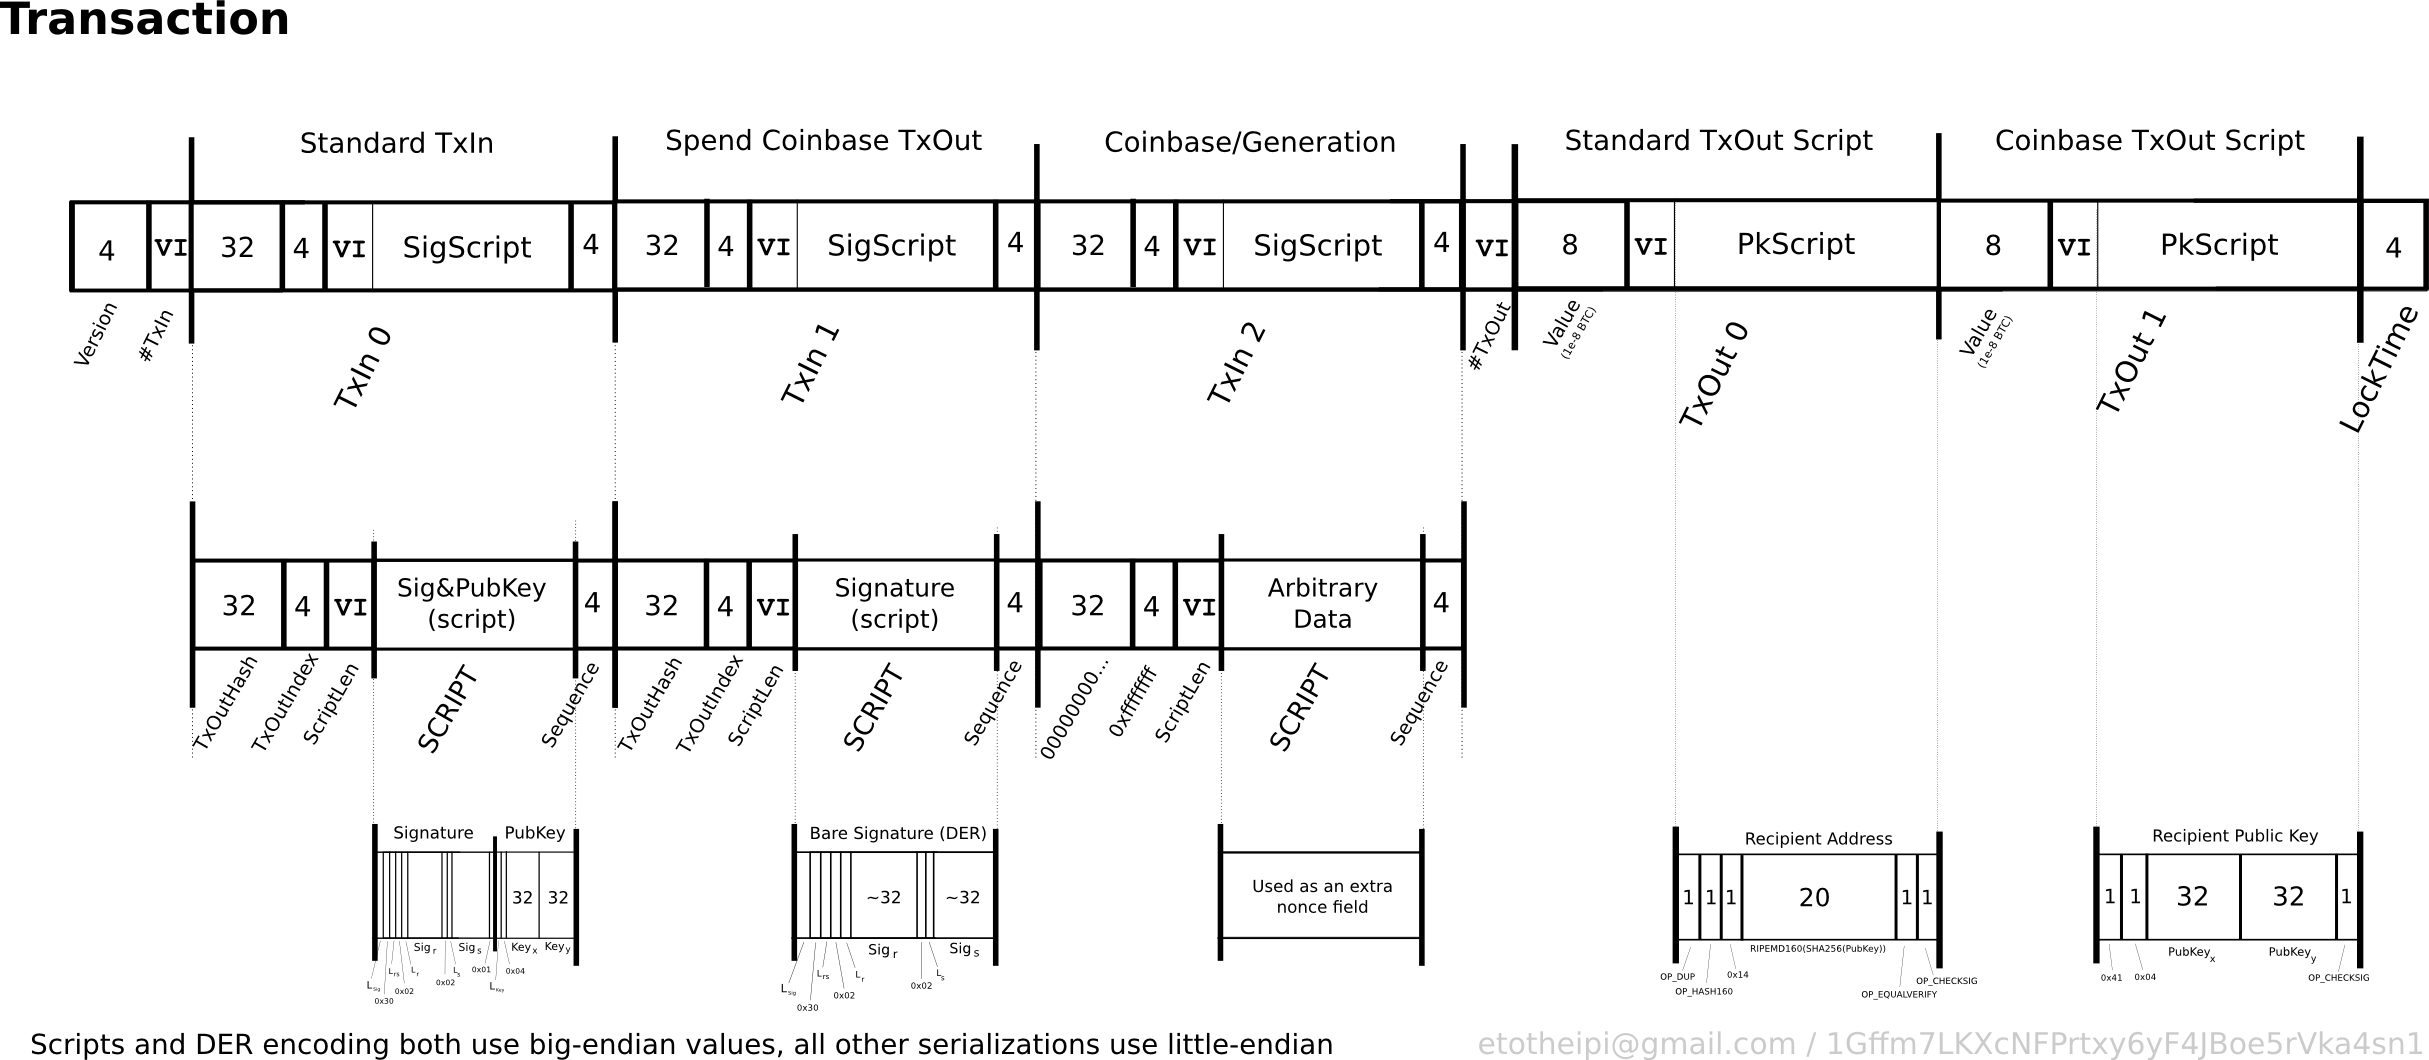
\includegraphics[width=\linewidth]{tx-binary}}
  \caption{A Bitcoin transaction in low-level, byte detail\cite{bitcoin_wiki_raw_tx:online}}}
  \label{fig:raw-tx}
\end{figure}

Understanding the version, number of inputs and outputs, references to outputs in inputs and specification of output values was mostly a reading task to know the byte format and encoding from the \textit{Bitcoin Wiki}\cite{bitcoin_wiki_tx:online}. Some fields like \textit{sequence} or \textit{locktime} were not researched depthly as were not relevant in that moment. The most difficult pieces to understand where the scripts, that specify how the transaction outputs can be spend and how the transaction inputs (that point to unspent outputs) get spent. 

\section{Script low-level understanding}
To understand scripts, the \textit{Bitcoin Wiki}\cite{bitcoin_wiki_script:online} provided very useful information about them in low-level, despite omitting (or not specifying clearly) details like the \textit{push data} opcodes. Several posts from forums, blogs and Q\&A answer sites where used to complete the information\cite{siliconian_raw_tx:online, stackoverflow_raw_tx:online}. The most difficult part was to understand how signatures are performed, since a new special transaction (copy of the transaction but removing some fields) has to be created to then sign it and set it into DER format in order to add a signature to a script\cite{bitcoin_wiki_sign:online, stackoverflow_signature_der:online}.

To view scripts in a more graphical way, the online site \textit{WebBTC} provided a visual script executor given a blockchain transaction\cite{webbtc_script:online} and \textit{hashmal} project from \textit{mazaclub} GitHub user provided a GUI to create and test scripts\cite{hashmal:online}.
\begin{figure}[H]
  \centering
  \makebox[\textwidth]{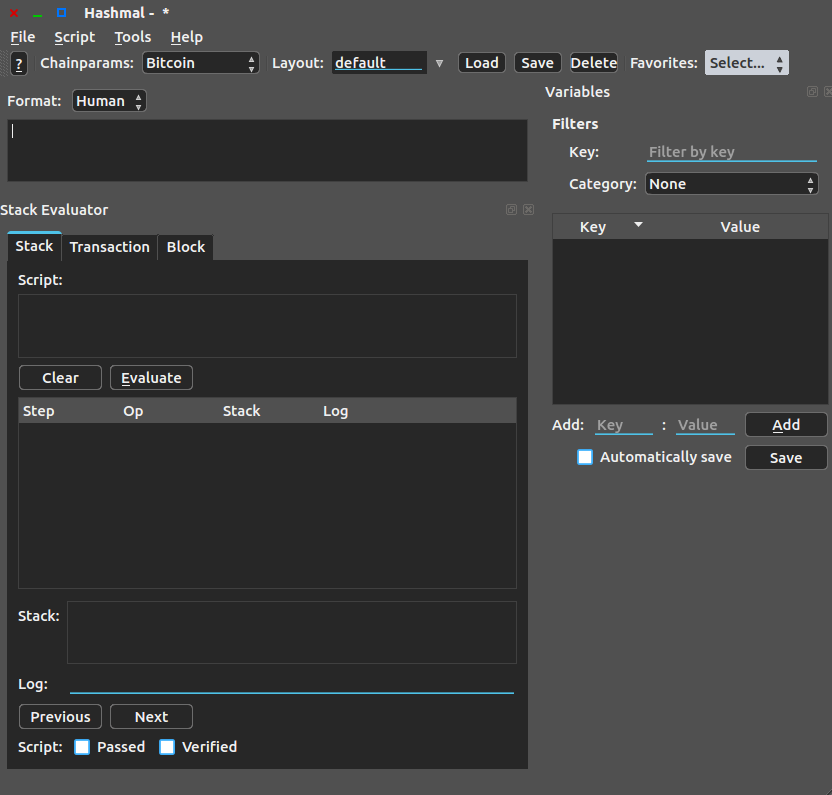
\includegraphics[width=\linewidth]{hashmal}}
  \caption{\textit{Hashmal} script editor and executor screenshot}
  \label{fig:hashmal}
\end{figure}

\section{Conclusions about the research}
Once the research was concluded and a raw transaction in bytes had acquired meaning for us, being able to decode most of the bytes in it, we concluded several points:
\begin{itemize}
    \item \textbf{The Bitcoin and \textit{smart contracts} potential}\\
    The fact that Bitcoin allows scripts to set how the funds of a transactions can be spent and scripts to spend those funds providing the conditions specified, has an enormous potential as allows developing \textit{smart contracts} that ables us to perform financial transactions with a huge set of possible spending conditions just limited to the scripting language limits, where those transactions will be protected cryptographically by a decentralized network of nodes that will check and validate that those conditions are accomplished. These idea and its potential has never seen before the appearance of Bitcoin.
    \item \textbf{Sparsed and few low-level documentation}\\ Despite there's quite much information about the Bitcoin concept and high-level operation explanations, there are just few websites that explain how Bitcoin works at a low-level detail, explaining what each byte means inside a transaction. Even best way to understand some details is to look at the Bitcoin Core's C++ implementation\cite{bitcoin_github:online}, the widely used Bitcoin node (with some comments that try to make the code more readable). Developing an informative website or media that collects and explains Bitcoin from the highest to the lowest level would be a really interesting and valuable educational resource that could aim more developers to play with the Bitcoin technology
    \item \textbf{The need for software models and architectures (ie: a framework)}\\ Due to the lots of concepts, ideas and dispersed items that play a role in Bitcoin (and just knowing and fully-understanding the transactions and therefore script pieces), defining a model (an object in OOP) for each item that is present in the process of a transaction generation can be a way to allow faster features development by abstracting hard low-level details so new developers don't get afraid to develop new Bitcoin features without spending hours to understand absolutely everything and losing time with technical, technological, programming-language details that don't provide any value or innovation. We'll try to create those models as much as our timing and project scope allows us to create them without delaying the schedule.\\ In this sense, the alt-currency Ethereum\cite{ethereum:online} has made great progress.
\end{itemize}
\setcounter{chapter}{3}
\setcounter{section}{0}
\chapter*{The software framework}
\addcontentsline{toc}{chapter}{The software framework}
\label{chap:software_framework}
Once the research was full-filled and (most part of) transactions were understood at a byte low-level, we started developing our software. 
\section{The goals}
The main goal for our software was to create simple P2PKH transactions in this first iteration of the development, to then be able to perform more iterations and add more complex transactions, until completing the project goal of creating the transactions needed to create and operate \textit{Bitcoin Payment Channels}.
\section{Technologies and environment setup}
We decided to use \textit{Python 3.6} because of our experience developing applications using this programming language and the ability it provides to focus on adding and implementing features quickly without having to worry much about low-level coding aspects like memory handling, centering the efforts in adding value to the application and therefore, to the project.

\subsection{Libraries}
After deciding the programming language, we searched for libraries that helped us performing complex operations like signatures, encoding operations, ...\\\\
We used the following ones:
\begin{itemize}
    \item \textbf{python-bitcoinlib\cite{python-bitcoinlib:online}}\\
    Provides handling of base58 encoding, scripts, public keys and data structures in general of the Bitcoin protocol
    \item \textbf{pybitcointools\cite{pybitcointools:online}}\\
    Library to perform common cryptographic operations in Bitcoin, providing an easy interface that converts the format of the input parameters automatically to avoid tedious format conversions
\end{itemize}

\subsection{Version control system}
We use Git, as mentioned in the initial report to handle the software versions and work in parallel. The source code of the project is publicly available\footnote{Checkout \url{https://www.uab.codes} to stay informed about the latest releases}:
\begin{center}
\url{https://github.com/uab-projects/btc-payment-channels}\footnote{Ensure to check the \code{development} branch as we don't spend time launching \textit{releases} very often as the code it's in continuous progress}
\end{center}

\section{The architecture and design}
As we said in the previous research chapter conclusions, there was a need of modelling the Bitcoin items in order to provide a better understanding and an abstraction to allow fast feature development without having to worry for low-level programming-language details. Following this non-functional requirements in aim to provide a better library for Bitcoin Python developers, we modelled all items that were in the scope of the project using OOP:
\begin{itemize}
    \item \textbf{Address}\\ An address allows to set how the funds must be spent in a transaction output, and can also contain public or private keys. Our model must provide an easy interface to create them using the items that they require, depending on the address type, that we'll also model. From an address, we have to be able to create automatically an output script if the address type matches (ie: does not contain a public / private key)
    \item \textbf{Script}\\ A script must be able to contain a list of fields (opcodes an data fields) to be able to set the spend conditions or to spend some output script. Therefore we can model a basic script, input, output, redeem and payment scripts and use the factory design pattern to easily build the most known types.
    \item \textbf{Input}\\ Contains the reference to the previous transaction, number of output, spending script, and sequence field
    \item \textbf{Output}\\ Contains the value to spend and the script with the conditions to spend
    \item \textbf{Transaction} \\ Contains all the transaction fields, version, inputs, outputs and locktime field
\end{itemize}
With all these items modelled and handled with easy, defining all formats of inputs and ouputs in an extensive in-code documentation, we provide a very good framework to work with and easily extend it using the items to create new transactions. We just have to have a way to transform them into bytes.
\subsection{The serializable interface}
To allow modularity and the easy combination of all the models, each of it must implement the serializable interface, that basically means that the object has to be able to be converted into an array of bytes (a \textit{bytes} built-in object in Python), with the \code{serialize()} method. Optionally (as it's not a feature to accomplish our project main goals), also has to implement a \code{deserialize} method, to create a new object from an array of bytes.\\\\
This way, we can create several objects from our models and join them as if we joined arrays of bytes, but with the ease of creation of a built-in Python classes instantiation, friendly for developers.
\subsection{The libraries' use}
If all these models have been created, why have we mentioned the previous libraries? We have just coded the models and joined them together, but the algorithmic parts and complex operations have been delegated to those libraries, such as base58 encoding and decoding for addresses and ECDSA signatures. The rest has been coded by ourselves.
\section{A basic transaction creation}
Once all the models have been coded and its serialization implemented, we have tested our framework by creating a P2PKH basic transaction that transfers funds creating a signature and setting the public key (hash) to pay to.\\\\ After several ECDSA signatures format mistakes and misunderstandings, we succesfully broadcasted a valid and confirmed transaction moving funds between ourselves.\footnote{The transaction can bee seen in the following \textit{testnet} block explorer using its \code{txId}: \url{https://tbtc.blockr.io/tx/info/258fb211724412d6ec6a531973c58233143e6ab355623658adc3164a5c70bd5b}}
The transaction was created before the milestone deadline scheduled, the 20th of March of 2017
\setcounter{chapter}{4}
\setcounter{section}{0}
\chapter*{Unidirectional payment channel}
\addcontentsline{toc}{chapter}{Unidirectional payment channel}
\label{chap:unidir-pc}
Once we can create transactions and more important, scripts, in an easy way, we are prepared to design more complex scripts to create \textit{smart contracts}. This means in the following iteration of development, we have to provide new models that allow the generation of \textit{multisig} redeem scripts and other special conditions like \textit{time / expire} conditions or \textit{hashlock} contracts.

\section{Understanding a payment channel}
There's quite few information about payment channels over Bitcoin cryptocurrency online. We've used the knowledge our tutors have provided us and an article also referenced by them on the \textit{Bitcoin Magazine}\cite{bitcoin_magazine_bidir_pc:online}.\\\\
The basics of a payment channel is that there has to be a \textit{commitment} or \textit{funding} transaction to fund the channel and then make payments using those funds to generate transactions that share out the funds to give more funds to a party. After the channel operation, the channel must be closed with a \textit{closing} transaction. \\\\
The idea is that those transactions that share out the funds can end in the blockchain (maybe after some time) and be valid, so that both nodes trust the transaction and can verify them using their nodes. But they don't get broadcasted to the network until the close transaction sets the final funds distribution, relieving the blockchain from storing those transactions and allowing to increase the speed of transactions between these parties as they can be generated and validated in much less time than the time it takes a regular transaction to appear on the blockchain and confirmed. At the time they exchange the payment transaction (that distributes the channel funds) the payment has been done as they know, can validate theirselves and trust that if the transaction ends in the blockchain would be valid.\\\\
The key is how to create those transactions in order that no attacks are possible (even DoS) to the channel by any of the parties by using cryptography and game theory
\section{Modelling a unidirectional payment channel}
Knowing that a payment channel implies the creation of scripts that ensure no attacks on the channel are possible and the parties play fair, the effort and problem is to create those scripts to be functional and secure at the same time. To speed up development, we will evade the malleability issues and assume the same scripts can be coded using \code{SegWit}, but without implementing them using \code{SegWit} to save time.
\subsection{Schedule problems}
At the time of writing this document, the schedule said we should have implemented those three scripts and transactions to allow \textit{commitment}, \textit{payment} and channel \textit{closure}. Due to the lack of awareness and excess of optimism, we couldn't design all three scripts and we just modelled the first one. In the rescheduling chapter, more details are given about how the schedule has changed.
\subsection{Commitment}
The commitment for a unidirectional channel can be done in two ways: a transaction that funds the channel and expires at a certain time, returning the funds to the funder(s) to prevent the funds from being locked out if a party doesn't collaborate or create a simple funding transaction and after that a refund transaction that is valid after a certain time. The easiest is two create two transactions, but triggers problems of who signs the transaction first, trust problems in the timelapse the first transaction is created and signed and the refund is signed too, .... The first option requires a complex script but avoids such trust problems
\subsubsection{Single-transaction commitment script}
This transaction funding transaction must spend inputs owned by the parties of the channel and set the output conditions to a \textit{multisig} output that requires both parties signatures to create transactions on, therefore creating the channel, or to return the funds after a certain time in order to prevent fund-locking if a party doesn't collaborate.

Creating a \textit{multisig} script requires the comprehension of Bitcoin P2SH scripts, that as many low-level aspects of the Bitcoin subject, few information can be found over the Internet. Fortunately, a blogger and developer posted a really detailed and clear explanation about the subject\cite{soroushjp_multisig:online}

Our \code{scriptSig} proposal for the payment transaction (whose partial hash, just of the redeemScript piece, would define the first commitment transaction using a P2SH).
\begin{center}
\code{OP\_0 <sigA> <sigB> | OP\_2 <pubKeyA> <pubKeyB> OP\_2 OP\_NOTIF <time> OP\_CHECKLOCKTIMEVERIFY OP\_DROP <PubKeyFunder> OP\_CHECKSIG}
\end{center}
Where \code{<PubKeyFunder>} would be the public key of the channel funder (we assume an easy case where just one of the parties fund the channel). In the case the channel expires, the \code{scriptSig} would change to spend the funds from \code{OP\_0 <sigA> <sigB>} to \code{OP\_0 <sigFunder> OP\_DUP OP\_OVER} so the \textit{multisig} fails but doesn't triggers and error and then the time is verified and after that the signature is checked agains the funder public key. This script has been revised by one of our tutors and requires its implementation and further testing
\setcounter{chapter}{5}
\setcounter{section}{0}
\chapter*{Goals revision}
\addcontentsline{toc}{chapter}{Goals revision}
\label{chap:goals-revision}
As appeared on the initial report, the final goal is to implement a bidirectional payment channel based on the idea and protocol explained on the Christian Decker's paper \cite{decker2015fast}. The software that implements the payment channel must be able to create a payment channel asking the user for parameters that can be understable for a person with basic Bitcoin knowledge about its operation.\\\\
Depending on the timing, that has changed due to optimistic estimations, we'll achieve a certain level of automation and ease to create the channel. We don't know how many iterations of software development (transaction model, script model, implementation and test) will take until the payment channel gets implemented and its operational. After that, the rest of cycles or iterations will be dedicated to automate and enforce the channel security. 

\section{Conclusion}
Despite the new and advanced low-level knowledge of Bitcoin that has made us reschedule the timing due to optimistic timings, we still think that can achieve the main goal of creating an operational bidirectional payment channel using the Christian Decker's protocol. What will change is that the automation and ease of use of the channel maybe won't be the same as the expected in the initial report.
\setcounter{chapter}{6}
\setcounter{section}{0}
\chapter*{Methodology revision}
\addcontentsline{toc}{chapter}{Methodology revision}
\label{chap:methodology-revision}
We thought at the initial report to work using a CVS for our code that we'll keep using as provides extended control and integrity over our code and iterative development as provides features in short periods of time, but taking an adequate time to design, implement and test (from now on transactions for the payment channels) and reducing the iteration times to one week or less strictly to see results soon. What we've learned is that design (or transaction and script model or creation in these cases) is really important as if a mistake is made in that stage and then everything gets implemented, we'll realize the mistake while testing, having to change the design and losing much of the time of a work that in most cases won't be profitable. Therefore in these further iterations of the software development we'll increase time in design and testing and try to reduce it in implementation as the prior objective is to create operational transactions that create a payment channel.

\section{Conclusions}
We'll follow the same methodologies as have been useful to keep and maintain a rhythm to be on time in most of the time of the project. We'll just invest a few more time in design stage to prevent design errors to be discovered on the test phase and losing implementation work time, while also adding more time to the test phase as implementing scripts is not easy as far as we have seen. Also reducing the iterations to one week or less will try to provide more features in less time. We'll check in next report how this methodology has worked.
\setcounter{chapter}{7}
\setcounter{section}{0}
\chapter*{Schedule revision}
\addcontentsline{toc}{chapter}{Schedule revision}
\label{chap:schedule-revision}
As we said before, and once our knowledge of Bitcoin arrived at a low-level detail, we realized the time we estimated for script and transaction modelling was too optimistic so changes appeared in the planning from that task forward.
\section{Changes motivation}
As appears in the previous methodology chapter, we'll dedicate more time to transaction modelling and script creation and to its testing and try to reduce the implementation time as with the framework created it will suppose to be simple and not require much lines of code. This way we want to achieve the goal by redistributing the time assigned to its task.
\section{Other minor changes}
In order to make the Gantt diagram simpler, we've reduced the iteration to design, implement, test and launch that mean to create, implement, test and broadcast transactions respectively. Therefore it's understood that in each iteration cycle, a different transaction will be developed, requiring 3 transactions modelling per channel (and that the unidirectional channel has to be implemented). Also several subtasks were reduced to a main task to reduce the resulting Gantt diagram size and iterations were defined to fullfill all diagram timelapse.
\clearpage
\section{Resulting Gantt diagram}
After performing the previously mentioned changes, we obtain the following new Gantt diagram:
\begin{figure}[ht]
  \centering
  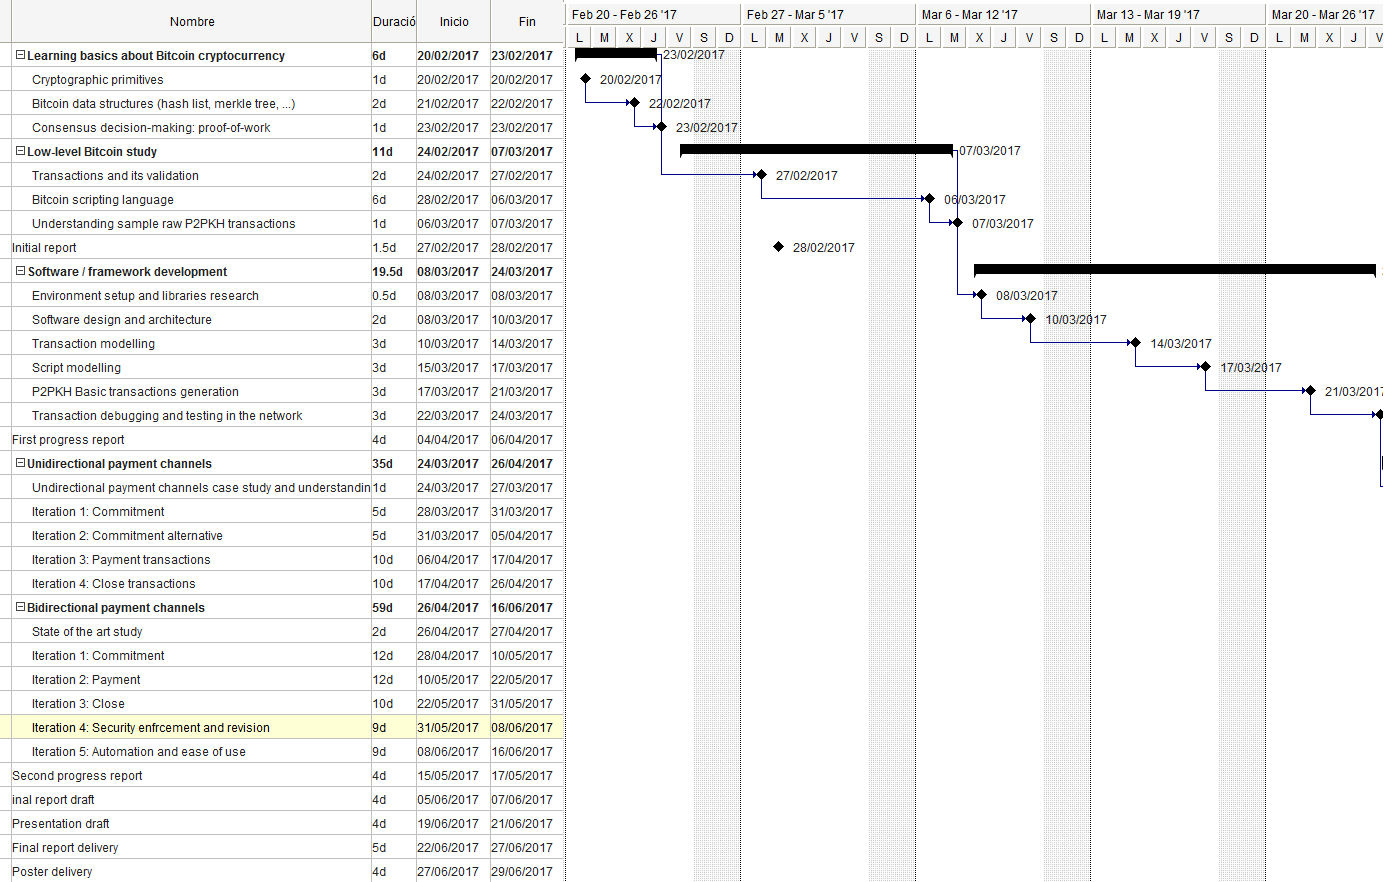
\includegraphics[width=\linewidth]{tasks-feb-mar.png}
  \caption{Gantt diagram of the new schedule [February-March]}
  \label{fig:gantt-diagram-feb-mar}
\end{figure}
\begin{figure}[ht]
  \centering
  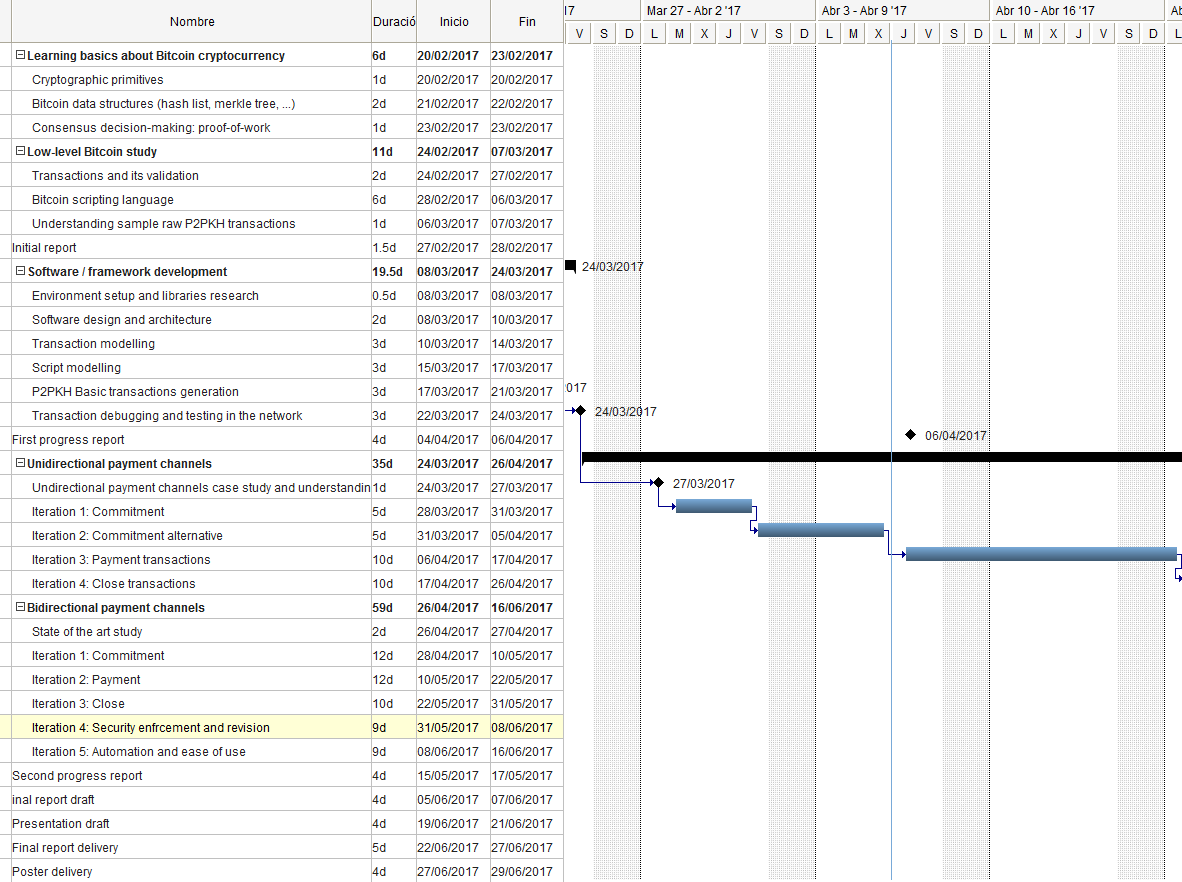
\includegraphics[width=\linewidth]{tasks-mar-apr.png}
  \caption{Gantt diagram of the new schedule [March - April]}
  \label{fig:gantt-diagram-mar-apr}
\end{figure}
\begin{figure}[ht]
  \centering
  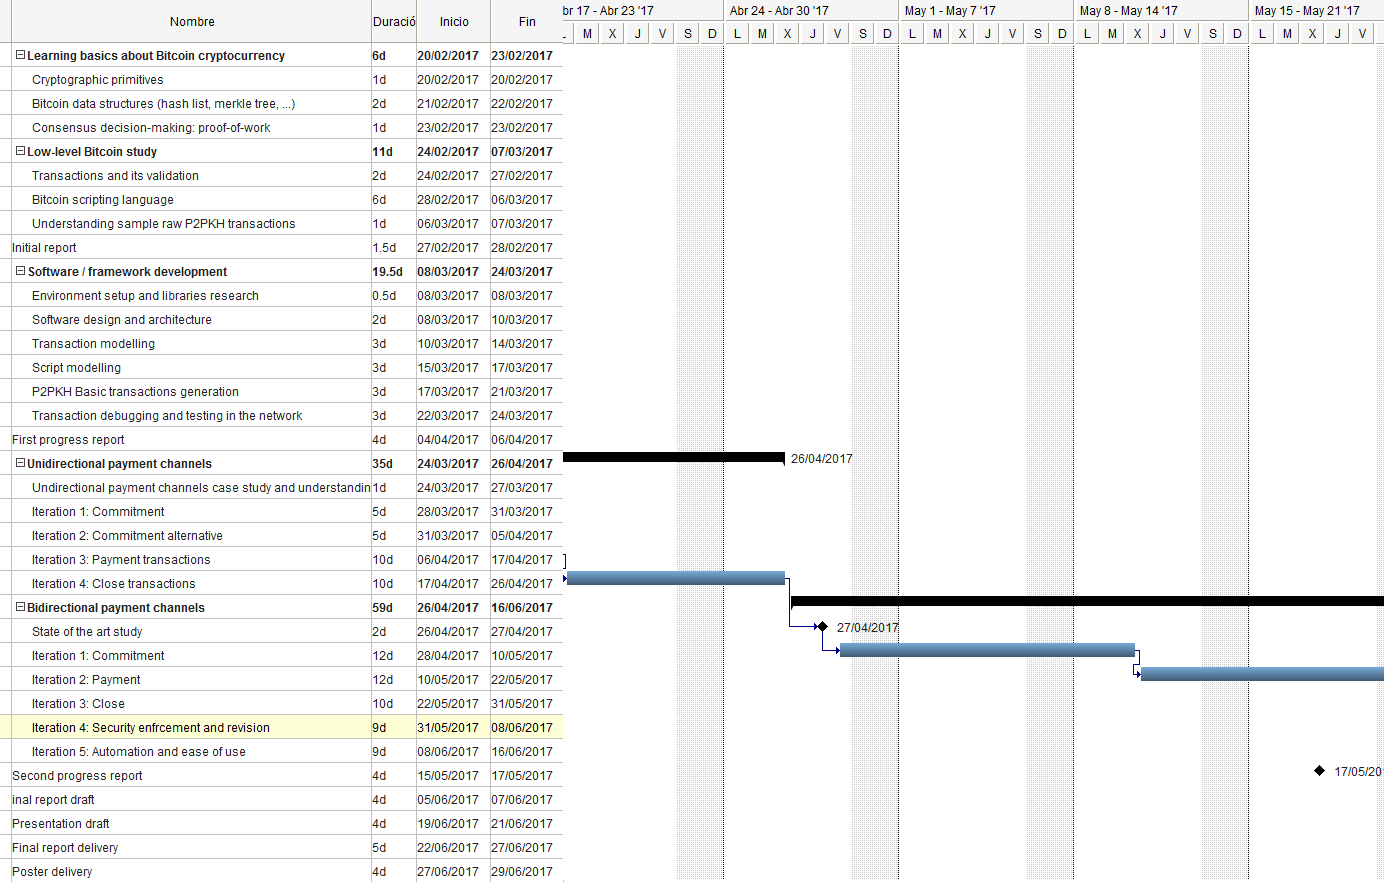
\includegraphics[width=\linewidth]{tasks-apr-may.png}
  \caption{Gantt diagram of the new schedule [April - May]}
  \label{fig:gantt-diagram-apr-may}
\end{figure}
\begin{figure}[ht]
  \centering
  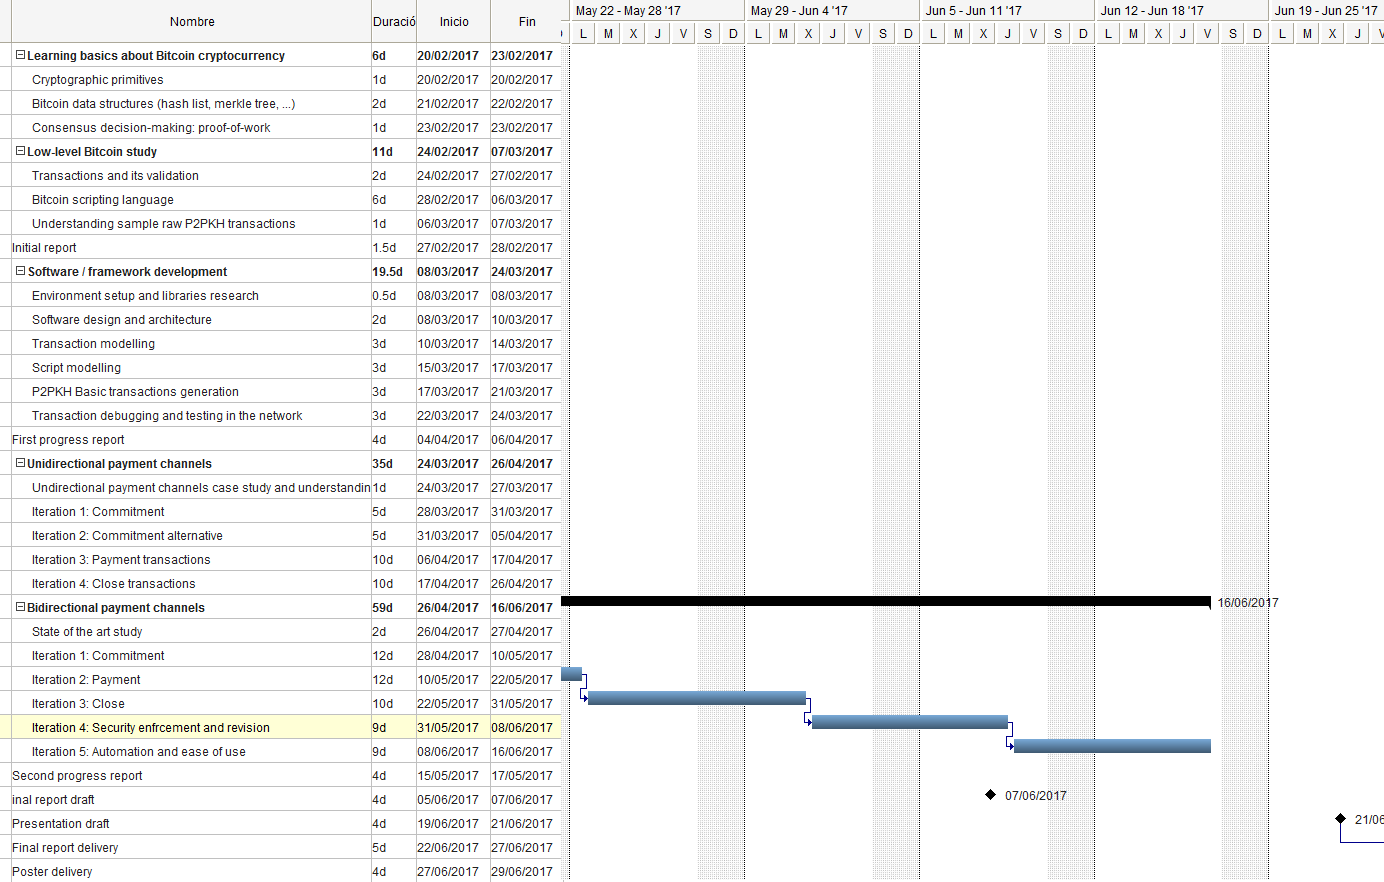
\includegraphics[width=\linewidth]{tasks-may-jun.png}
  \caption{Gantt diagram of the new schedule [May - June]}
  \label{fig:gantt-diagram-may-jun}
\end{figure}
\begin{figure}[ht]
  \centering
  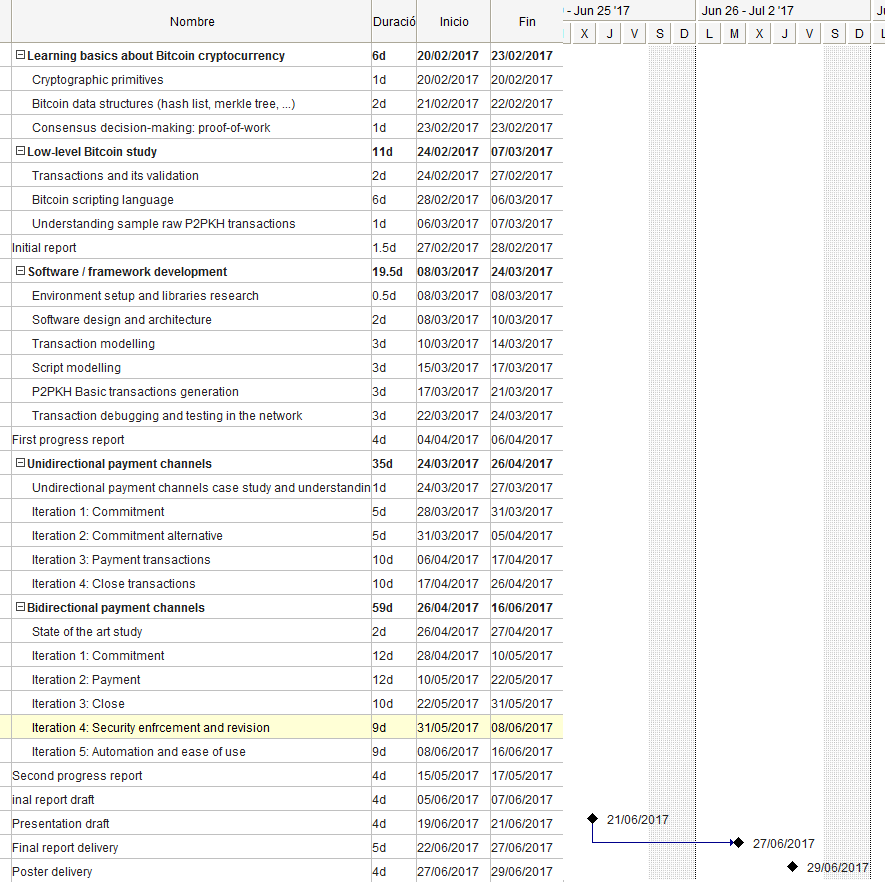
\includegraphics[width=\linewidth]{tasks-end.png}
  \caption{Gantt diagram of the new schedule [June - end]}
  \label{fig:gantt-diagram-end}
\end{figure}

\appendix

%%%%%%%%%%%%%%%%%%%%
%%% Bibliography %%%
%%%%%%%%%%%%%%%%%%%%

\bibliographystyle{ieeetr}
\bibliography{references}

\clearpage

%%%%%%%%%%%%%%%%
%%% Abstract %%%
%%%%%%%%%%%%%%%%

%\thispagestyle{empty}
%\topskip0pt
%\vspace*{\fill}
%\noindent\rule[2pt]{\textwidth}{0.5pt}\\
%{\textbf{Summary}}
%Lorem ipsum dolor sit amet, consectetur adipiscing elit. Sed non risus. Suspendisse lectus tortor, dignissim sit amet, adipiscing nec, ultricies sed, dolor. Cras elementum ultrices diam. Maecenas ligula massa, varius a, semper congue, euismod non, mi. Proin porttitor, orci nec nonummy molestie, enim est eleifend mi, non fermentum diam nisl sit amet erat. Duis semper. Duis arcu massa, scelerisque vitae, consequat in, pretium a, enim. Pellentesque congue. Ut in risus volutpat libero pharetra tempor. Cras vestibulum bibendum augue. Praesent egestas leo in pede. Praesent blandit odio eu enim. Pellentesque sed dui ut augue blandit sodales. Vestibulum ante ipsum primis in faucibus orci luctus et ultrices posuere cubilia Curae; Aliquam nibh. Mauris ac mauris sed pede pellentesque fermentum. Maecenas adipiscing ante non diam sodales hendrerit. Ut velit mauris, egestas sed, gravida nec, ornare ut, mi. Aenean ut orci vel massa suscipit pulvinar. Nulla sollicitudin. Fusce varius, ligula non tempus aliquam, nunc turpis ullamcorper nibh, in tempus sapien eros vitae ligula. Pellentesque rhoncus nunc et augue. Integer id felis.
%\noindent\rule[2pt]{\textwidth}{0.5pt}
%\vspace*{\fill}
\end{document}